\subsubsection{\stid{5.01} Software Development Kits} \label{subsubsect:ecosystem-sdk}

\paragraph{Overview} The ST Software Development Kit (SDK) project supports a set of activities aimed at

\begin{itemize}
\item establishing Community Policies aimed at increasing the interoperability between and sustainability of ST software packages, using the xSDK community package~\cite{xSDK-community-package-policies2016} and installation~\cite{xSDK-community-installation-policies2016} policies as a model (reference to xSDK section?).

\item coordinating the delivery of a comprehensive and coherent set of software tools to all interested stakeholders on behalf of ECP ST. This includes ECP applications and the broader open source community.

\end{itemize}

SDK is needed within ECP because it will make it simpler for ECP applications to access required software dependencies on ECP target platforms and drastically lower the cost of exploring the use of additional ECP ST software that may be of benefit. In addition, the SDK effort will decrease the ECP software support burden at the major computing facilities by ensuring the general compatibility of ST packages within a single software environment, providing tool support for the installation of ST packages on facility machines, communicating common requirements for ST software and facilitating the set up of CI testing on facility platforms. This project will work closely with the HI 2.4.4 \textit{Deployment of Software at the Facilities} project.

\paragraph{Key  Challenges}
ST software packages have been developed in a variety of very different cultures and are at significantly different levels of software engineering maturity and sophistication. The experience of some of the SDK staff during the formation of the xSDK showed that in this situation, it is challenging to establish common terminology and effective communication, and these are prerequisites to community policies and a robust software release.

Deciding exactly how to deploy the SDKs at the facilities is itself a challenge. ECP applications will use different combinations of ST software in different configurations. For example, applications will want mathematical libraries capabilities from the xSDK build on top of both MPICH and OpenMPI, and will want different configurations of those mathematical libraries.

\paragraph{Solution Strategy}
The SDK solution strategy involves pursuing interoperability and sustainability goals by grouping ST software projects into logical collections whose members will benefit from a common set of community policies as well as increased communication between members to standardize approaches where sensible and establish better software practices. The SDK effort will also facilitate the use of common infrastructure, such as CI testing at the major computing facilities and the Spack~\cite{gamblin+:sc15} package manager.

SDK release and delivery goals will also benefit from common package manager and testing infrastructure. In addition to delivery through Spack, the SDK will also explore the option of binary delivery, possibly through OpenHPC.

Recognizing the different release readiness and broader maturity differences between different ECP ST products, the early release strategy is to include only those products ready for a joint release in the initial SDK release, but to also continue to work with other products in preparing for subsequent release opportunities.

\paragraph{Recent Progress}
The SDK team decided to use a horizontal as opposed to vertical approach for forming SDKs. A horizontal approach emphasizes the grouping of software according to function and purpose, such as MPI implementations, compiler frameworks, performance analysis, or mathematical libraries. A vertical approach would have grouped ST software products based on products that are built in a stack for end users. 

Figure~\ref{fig:sdk-horizontal} illustrates the horizontal relationship between ST products in an SDK. The packages shown in green are all members of the xSDK, and are all mathematical libraries software. Software shown in black are not xSDK member packages. However, OpenMPI is an ECP ST software package. Although OpenMPI is commonly used with xSDK member packages (a vertical relationship), it is not a mathematical library (a horizontal relationship), and is therefore not part of the xSDK.
\begin{figure}[htb]
        \centering
        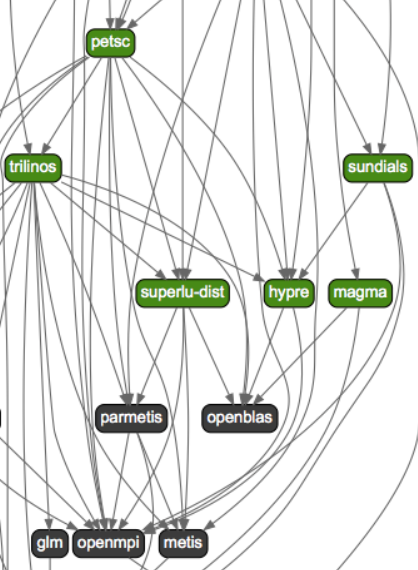
\includegraphics[width=2in]{projects/2.3.5-Ecosystem/2.3.5.01-Ecosystem-SDK/SDKfig}
        \caption{\label{fig:sdk-horizontal}The above diagram shows a snippet of the Spack dependency tree including six xSDK member packages. While multiple xSDK member packages depend on OpenMPI, which is an ECP ST software product, OpenMPI is not part of the xSDK}
\end{figure}


Some initial SDK groupings have been proposed based on the horizontal grouping approach. Lower level SDKs from the Programming Models and Runtimes area are available in a container environment for the purposes of supporting higher-level SDKs and testing SDK infrastructure.

\paragraph{Next Steps}
Current and near-term efforts include:

\begin{itemize}
\item  defining additional ST SDKs based on horizontal grouping principles.
\item  beginning regular requirements discussions with computing facilities.
\item  identifying resources and a plan for assisting ECP ST packages with Spack package creation (over 50\% already have a Spack package).
\item  beginning community policy discussions within SDK package teams.
\item  choosing a target set of ST products for inclusion in the FY19 Q1 release.
\end{itemize}

